\label{ch:method}
L'obiettivo di questo lavoro è dotare Knoxly di un modulo intelligente capace di comprendere la semantica di un testo scritto in linguaggio naturale (\textit{il testo parla di argomenti potenzialmente sensibili?}), comprendere se il testo che si sta per divulgare sul Web contiene dati sensibili o personali~\cite{dataSpectrum} (\textit{l'utente sta divulgando la propria opinione politica?}), inviare - nel caso - una notifica all'utente (privacy awareness), ed adattarsi alle esigenze dell'utente (alcuni utenti, es. esercenti fisici, potrebbero non essere interessati a ricevere notifiche riguardo la possibile divulgazione della loro location). Alla luce degli obiettivi, ci si è mossi verso tecniche basate su Intelligenza Artificiale che si sono mostrate utili in svariati contesti simili (si faccia riferimento, ad esempio, a~\cite{dontTweetThis, hybrid}).

\begin{figure}[h!t]
    \centering
    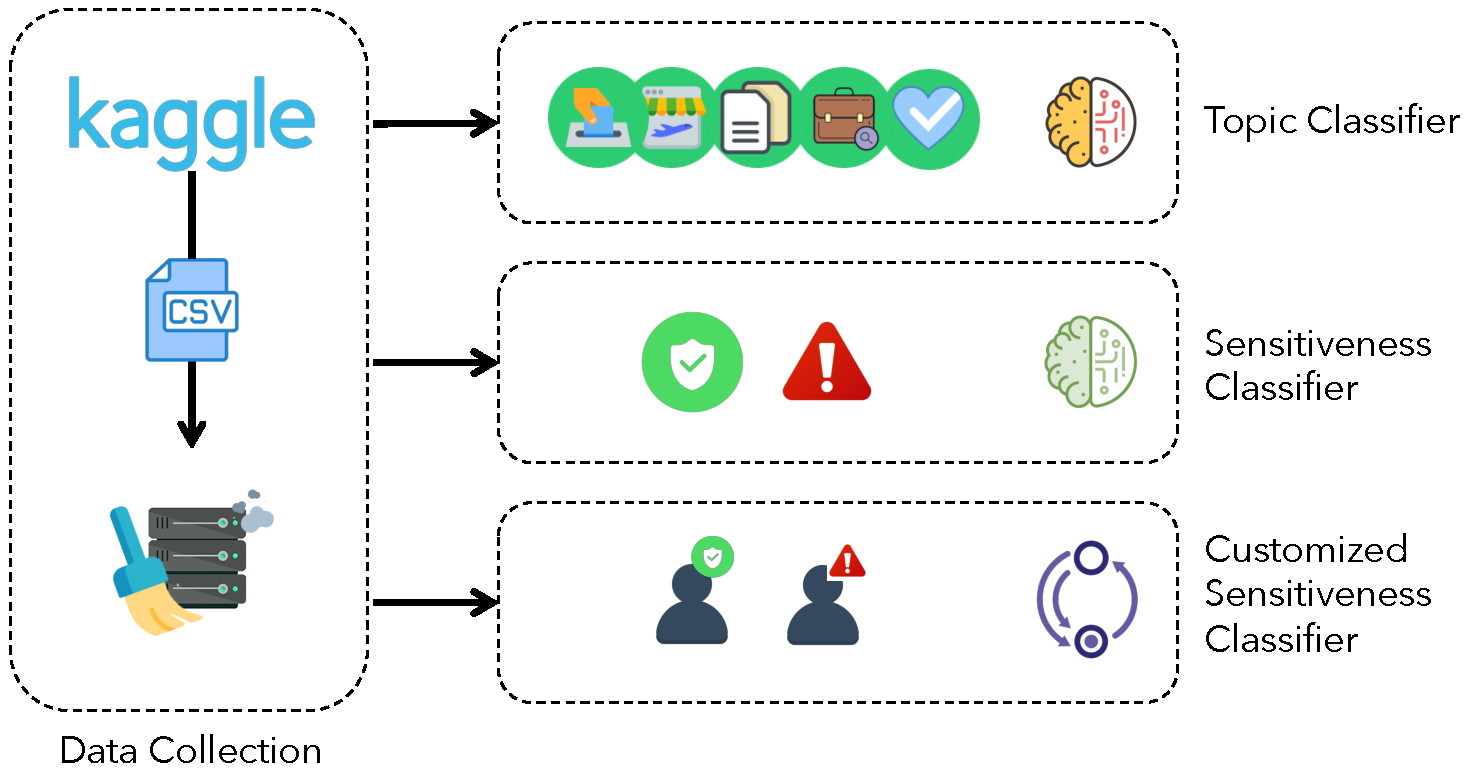
\includegraphics[width=15cm]{Figure/grafici/wholemethodology_cropped.pdf}
    \caption{Principali fasi della metodolgia adottata: (1) \textit{Data collection}, individuazione, raccolata e pre-processing dei dati utili alle fasi successive; \textit{(2) Topic classifier}, realizzare una modello che data una frase è in grado di riconoscere il topic di appartenenza; \textit{(3) Sensitiveness classifier}, realizzare un modello che data una frase è in grado di capire se contiene dati potenzialmente personali e sensibili; \textit{(4) Customized sensitiveness classifier}, realizzare un modello in grado di capire quali sono i dati sensibili per un utente adattandosi alla sua percezione di privacy.}
    \label{fig:wholemethod}
\end{figure}

Per realizzare il core intelligente di Knoxly è stata seguita una metodologia che si suddivide nelle seguenti fasi (vedi Figura~\ref{fig:wholemethod}):
\begin{itemize}
    \item Data collection (Sezione~\ref{datacollection}): individuazione, raccolta e pre-processing dei dati;
    \item Topic classifier (Sezione~\ref{sec:topicclass}): realizzare una modello che data una frase è in grado di riconoscere il topic di appartenenza;
    \item Sensitiveness classifier (Sezione~\ref{sec:sensclass}): realizzare un modello che data una frase è in grado di capire quanto essa sia sensibile;
    \item Customized sensitiveness classifier (Sezione~\ref{sec:pres_sens_class}): realizzare un modello in grado di capire quali siano i dati sensibili per un utente.
\end{itemize}



\section{Data collection}
\label{datacollection}
La prima fase del lavoro consiste nel collezionare i dati utili agli step successivi. Per creare il dataset su cui verranno addestrati i modelli di (a) \textit{Topic classifier}, (b) \textit{Sensitiveness classifier} e (c) \textit{customized sensitiveness classifier}, bisogna come prima cosa raccogliere i dati raw (non elaborati).
Sulla base di quanto spiegato nella sezione~\ref{ssec:sensitive_data} sono stati individuati quattro topic di particolare interesse: politica, viaggi, salute, lavoro, come fatto anche in~\cite{looseTweets,dontTweetThis,MalandrinoScarano}.

\begin{table}[h]

\centering
    \fontsize{4.6mm}{4.6mm}\selectfont{
    \renewcommand{\arraystretch}{1.4}
    \setlength\tabcolsep{4.0pt}
    \begin{tabular}{c|c|c|c}
    \toprule
    \textbf{Topic} & \textbf{nome dataset} & \textbf{Reference} & \textbf{\# entry} \\
    \midrule
    Politics & Election Day Tweets & \cite{ds_pol}  & 393.764 \\ \hline
    Health & Medical Transcriptions & \cite{ds_health1} & 2.348 \\ \hline
    Health & Medical Speech, Transcription, and Intent & \cite{ds_health2} & 706 \\ \hline
    Job & AMAZON Job Skills & \cite{ds_job} & 2.505 \\ \hline
    Travel & Twitter US Airline Sentiment & \cite{ds_travel} & 14.427 \\ \hline
    General & The Movies Dataset & \cite{ds_general} & 44.306 \\
    \bottomrule
    \end{tabular}
    }
\caption{Dataset scelti su Kaggle.com per ogni topic d'interesse.}
\label{tab:ds_scelti}
\end{table}
\FloatBarrier

Una volta definiti i topic, sono stati individuati dei dataset opportuni. In particolare, è stato effettuato il download di dataset messi a disposizione dal sito \href{https://www.kaggle.com/}{kaggle.com} i quali dopo una fase di pre-processing sono stati uniti in un unico \quotes{dataset raw}. Nella tabella~\ref{tab:ds_scelti} vengono mostrati i dataset selezionati per ogni topic con il relativo numero di elementi e il link per scaricarlo.

Si è deciso di introdurre un topic che chiameremo \quotes{General} il quale ci servirà per aumentare l'eterogeneità dei dati, creando rumore. È chiaro che un modello di machine learning basato solo sui topic potenzialmente ricchi di dati sensibili e personali, classificherebbe qualsiasi testo in una delle categorie individuate: ciò genererebbe misclassification perchè esistono dei testi che non ricadono in nessuna delle categorie tra health, politics, job e travel. Nel topic \quotes{General} sono contenute delle trame di film: sono state scelte le trame perchè queste sono composte da testi brevi e raccontano una storia e in alcuni casi questa può riportare dei dati sensibili e personali riguardo i personaggi.

I dataset scelti sono salvati come file {\tt .csv}: essi presentano diverse colonne, alcune di queste irrilevanti ai fini di questo lavoro.

\begin{table}[h!t]
\centering
\begin{tabular}{|l|c|l|}
\hline
\multicolumn{1}{|c|}{\textbf{Topic}} & \textbf{file} & \multicolumn{1}{c|}{\textbf{col. scelta}} \\ \hline
Politics & {\tt election\_day\_tweets.csv} & text \\ \hline
Health & {\tt mtsamples.csv} & description \\ \hline
Health & {\tt overview-of-recordings.csv} & phrase \\ \hline
Job & {\tt amazon\_jobs\_dataset.csv} & \begin{tabular}[c]{@{}l@{}}description,\\ basic qualifications,\\ preferred qualifications\end{tabular} \\ \hline
Travel & {\tt Tweets.csv} & text \\ \hline
General & {\tt movie\_metadata.csv} & overview \\ \hline
\end{tabular}
\caption{File e colonne (col. scelta) selezionate dai dataset di Kaggle}
\label{tab:col_scelte}
\end{table}
\FloatBarrier

In Tabella~\ref{tab:col_scelte} si elencano i file scelti e le colonne selezionate che comporranno il dataset.

\section{Pre-processing sui raw data}
\label{sec:preprocessingraw}
I testi selezionati risultano molto eterogenei quindi prima di raggruppare tutto in un unico dataset è stata necessaria una \quotes{pulizia} di questi dati.

Dai vari subset ricavati dai dataset originali di Kaggle sono state eliminate le righe che contenevano un testo di lunghezza $l<3$ caratteri e che non erano scritti in lingua inglese. La fase language detection è stata condotta utilizzando la libreria Python  TextBlob\footnote{\url{https://textblob.readthedocs.io/en/dev}}.

Si è notato che i testi nel dataset Job risultano essere particolarmente lunghi (lunghezza media degli annunci è di 968 caratteri, SD=788.40) e ciò può rappresentare un problema di conformità rispetto gli altri dataset considerati. Per ridurre le dimensioni delle singole entry appartenti alla categoria job si è deciso di dividere in varie parti l'annuncio di lavoro. Questa operazione è stata eseguita utilizzando il sentence splitter\footnote{\url{https://github.com/berkmancenter/mediacloud-sentence-splitter}}, fornito dai ricercatori Philipp Koehn e Josh Schroeder~\cite{Koehn07}. 

Terminata questa fase, i vari dataset processati sono pronti per essere uniti ed etichettati.

\section{Topic classification}
\label{sec:topicclass}
Il primo obiettivo del lavoro è la definizione ed implementazione di un modulo intelligente capace di comprendere la semantica di un testo scritto in linguaggio naturale, che sia in grado di capire di cosa l'utente sta parlando.

\begin{figure}[h!t]
    \centering
    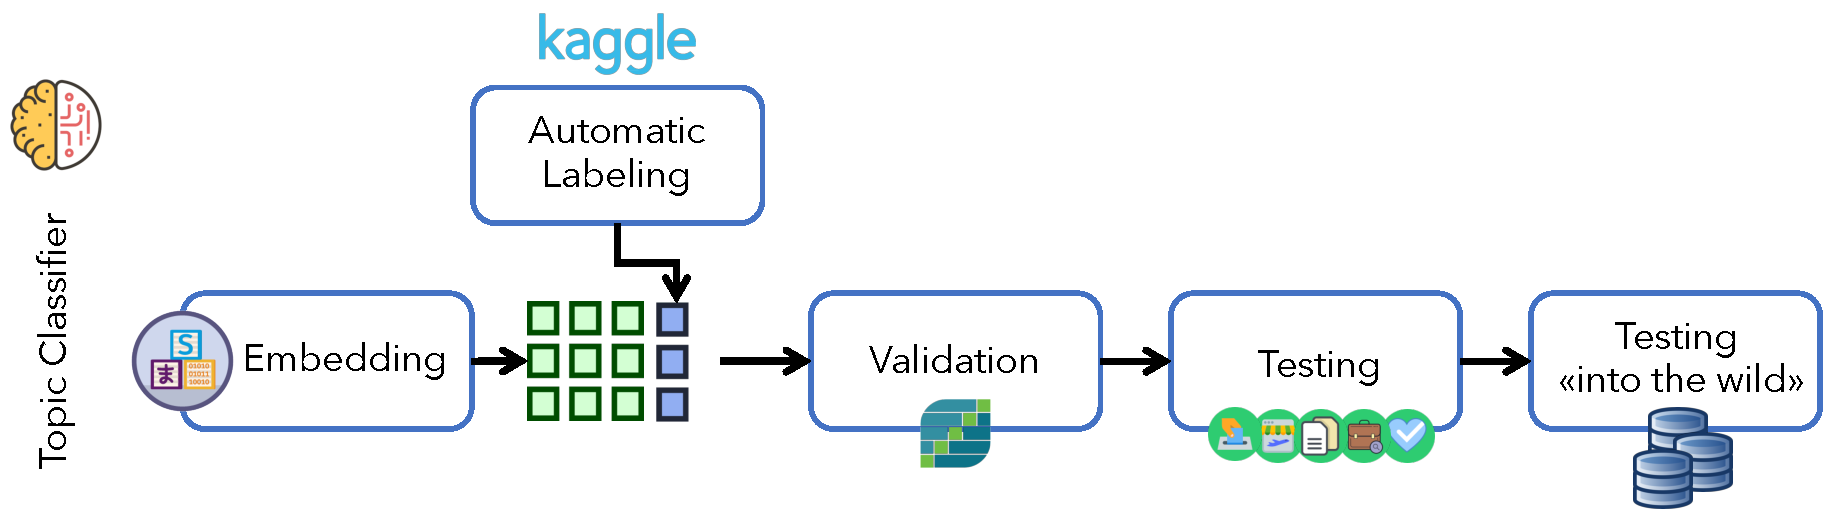
\includegraphics[width=15cm]{Figure/grafici/topicmethod_cropped.pdf}
    \caption{Principali fasi per la creazione del modulo Topic Classifier: (\textit{Embedding}) le frasi dei vari dataset vengono trasformate in vettori a lunghezza fissa; (\textit{Automatic Labeling}) in base al dataset di provenienza ciascun sample (embedding) viene etichettato automaticamente; (\textit{Validation}) mediante una k-fold cross-validation si validano vari classificatori basati sul supervised learning e si effettua il tuning degli iper-parametri utilizzando il training set $trs$; (\textit{Testing}) una volta ottenuti i migliori parametri per ciascun classificatore, si effettua il testing sul test set $tss$; (\textit{Testing \quotes{into the wild}}) si effettua un ulteriore testing su nuovi dati.}
    \label{fig:topicmethod}
\end{figure}

A tal fine è stata seguita una metodologia che consta nelle seguenti fasi (vedi Figura~\ref{fig:topicmethod}):
\begin{itemize}
    \item Creazione del dataset (Sezione~\ref{ssec:createds}): si illustra (a) la/e tecnica/che utilizzate per la conversione dei testi del dataset in vettori di numeri reali (sample) da dare in input al classificatore, (b) la strategia di labeling dei sample; 
    \item Validation (Sezione~\ref{ssec:validation_Topic}): validazione del modello realizzato utilizzando la k-fold cross-validation;
    \item Testing (Sezione~\ref{ssec:testing_Topic}): testing delle performance del metodo sul test set;
    \item Testing~\quotes{into the wild} (Sezione~\ref{ssec:testing_wild}): ulteriore testing delle performance del metodo, su un dataset molto più ampio.
\end{itemize}

\subsection{Creazione del dataset}
\label{ssec:createds}
Una volta ultimata la fase di pre-processing i dati sono stati uniti in unico dataset composto da 2426861 elementi. Per questo esperimento abbiamo deciso di utilizzare un subset di questo dataset, composto da 1000 elementi per ciascun topic, selezionati con una funzione {\tt random}. Successivamente si è passati alla fase di rappresentazione del testo (Sezione~\ref{sssec:rappresentazione}) e labeling (Sezione~\ref{sssec:textlabeling}).

\subsubsection{Rappresentazione del testo}
\label{sssec:rappresentazione}
Per rappresentare i testi è stato utilizzato USE di Google (vedi Sezione~\ref{sec:use}), perchè si ipotizza che le frasi appartenenti allo stesso topic siano simili fra loro e di conseguenza anche i vettori risultanti dall'operazione di embedding saranno simili. Ogni testo viene quindi convertito in un array di 512 elementi. Per mostrare la validità di questa ipotesi è stato selezionato un campione {\tt random} di 5 frasi per ogni topic, è stato effettuato l'embed delle frasi e poi calcolato l'inner product degli embed. L'inner product è una tecnica molto semplice per comprendere la similarità tra due vettori. Il valore di similarità $s \in [0..1]$, dove $1$ indica frasi / vettori identiche / ci, $0$ indica completa dissimilarità, quindi più il valore è vicino a $1$ più le / i frasi / vettori sono simili.

Di seguito vengono mostrate le matrici di similarità ottenute dell'inner product. Si può notare che le matrici di similarità con i valori più alti sono politics (Figura~\ref{fig:mtrsim_p}) - con valori che vanno da 0.63 a 1 -, job (Figura~\ref{fig:mtrsim_j}) - con valori che vanno da 0.72 a 1.

Infine, è stata realizzata una matrice che mette insieme le frasi selezionate per ciascun topic per valutare quanto queste se appartenenti a diversi topic si somiglino (differiscano tra loro in questo caso). Il risultato è mostrato in (Figura~\ref{fig:mtrsim_mix}) dove si può notare che le celle colorate con toni chiari (valori superiori a 0.5) siano ottenute dalla intersezione di frasi appartenenti allo stesso topic, mentre, le celle colorate con toni scuri (valori inferiori al 0.5) siano date dell'inner product di frasi appartenenti a topic diversi.

\begin{figure}[h!t]
    \centering
    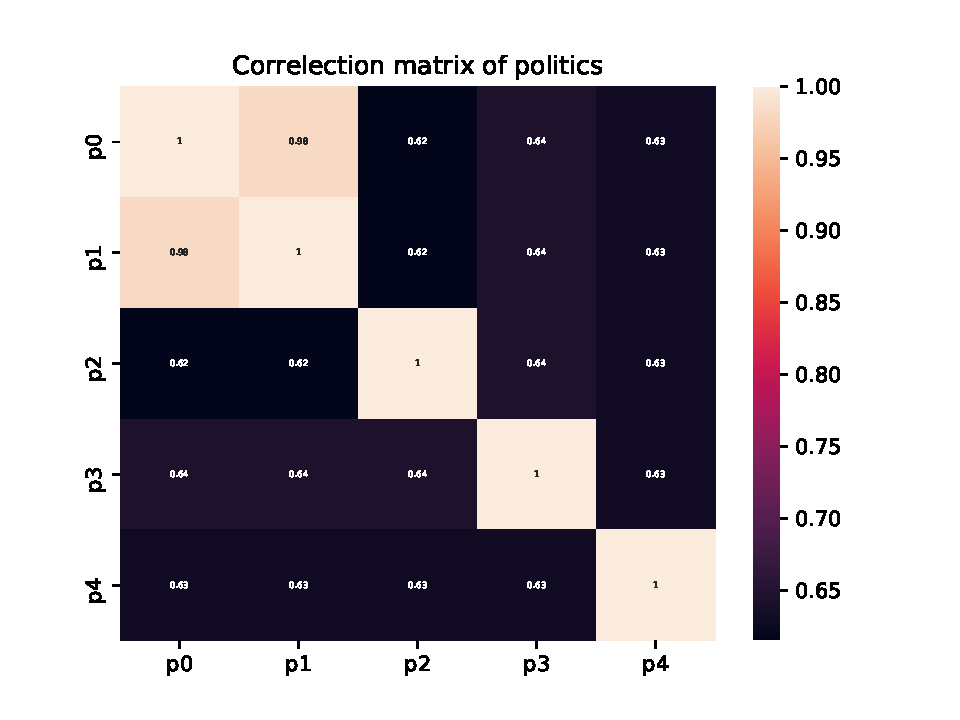
\includegraphics{Figure/simMatr/politics.pdf}
    \caption{matrici di similarità delle frasi appartenenti al topic politics. Dal campione di 5 frasi preso in esame per il topic poltics si può notare che tutte la maggior parte delle coppie(escludendo le coppie poste sulla diagonale principale) hanno una similarità che va da 0.62 a 0. 64, tranne per la coppia [p1, p0] dove si può notare una similarità pari a 0.98.}
    \label{fig:mtrsim_p}
\end{figure}
\FloatBarrier

\begin{figure}[h!t]
    \centering
    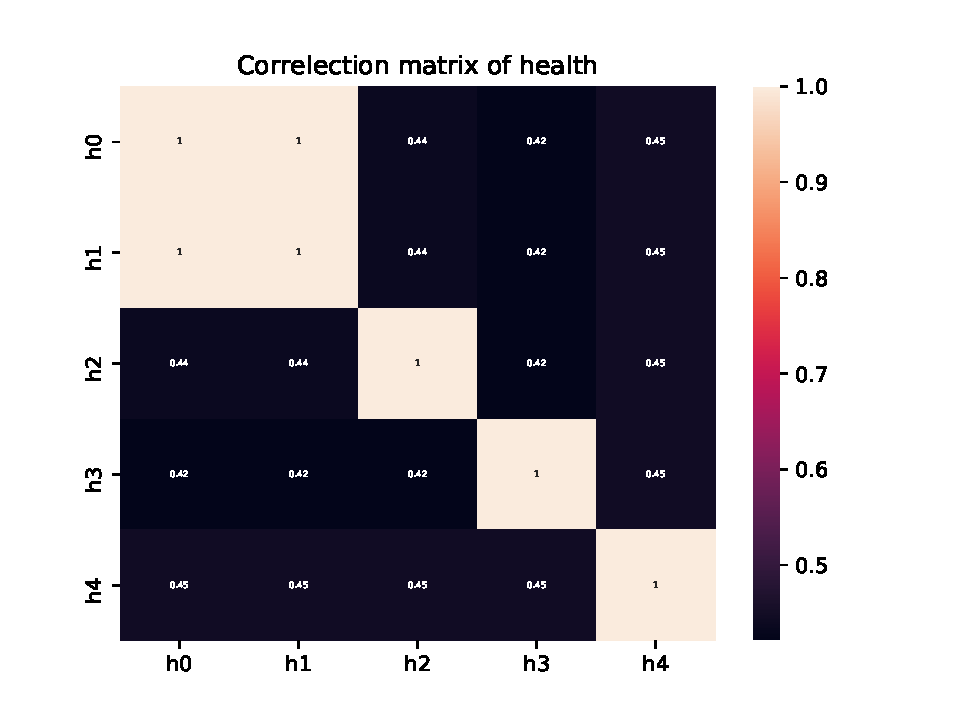
\includegraphics{Figure/simMatr/health.pdf}
    \caption{matrici di similarità delle frasi appartenenti al topic health. Dal topic health si può notare che le frasi sono poco simili fra loro infatti(escludendo le coppie sulla diagonale principale) tutte le coppie tranne la coppia[h1, h0] hanno una similarità compresa fra 0.42 e 0.45. La coppia [h1, h0] ha una similarità pari a 1 questo significa che nelle frasi appartenenti al topic health una singola frase può avere più di una sola occorrenza.}
    \label{fig:mtrsim_h}
\end{figure}
\FloatBarrier

\begin{figure}[h!t]
    \centering
    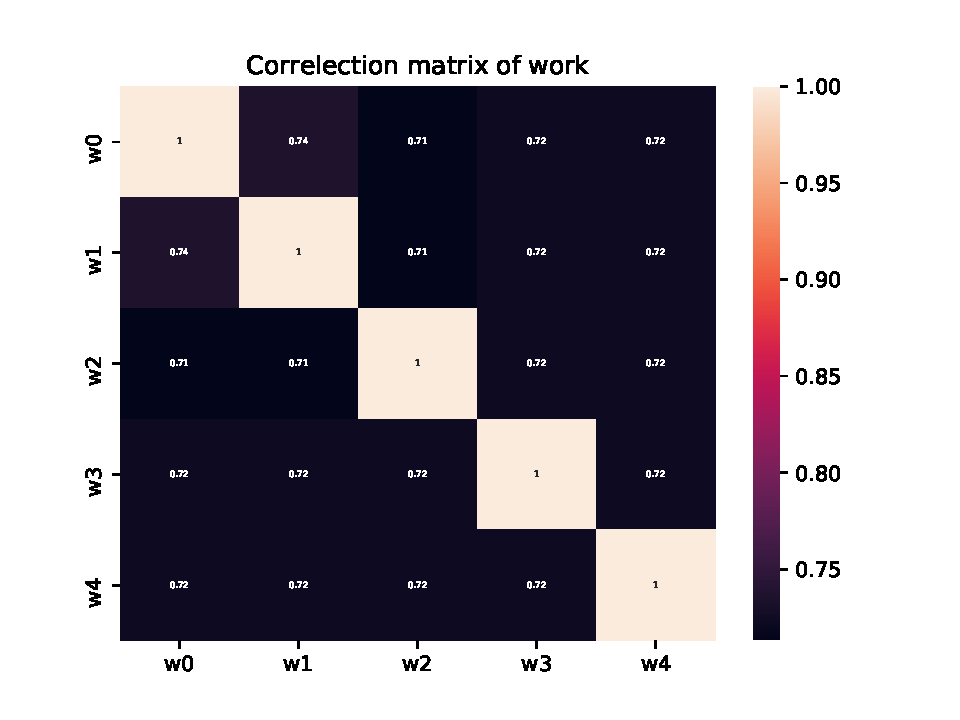
\includegraphics{Figure/simMatr/work.pdf}
    \caption{matrici di similarità delle frasi appartenenti al topic job. Il topic job è il topic che ha i valori di similarità più alti, infatti, tutte le coppie(escludendo quelle sulla diagonale principale) hanno una similarità compresa fra 0.71 e 0.74.}
    \label{fig:mtrsim_j}
\end{figure}
\FloatBarrier

\begin{figure}[h!t]
    \centering
    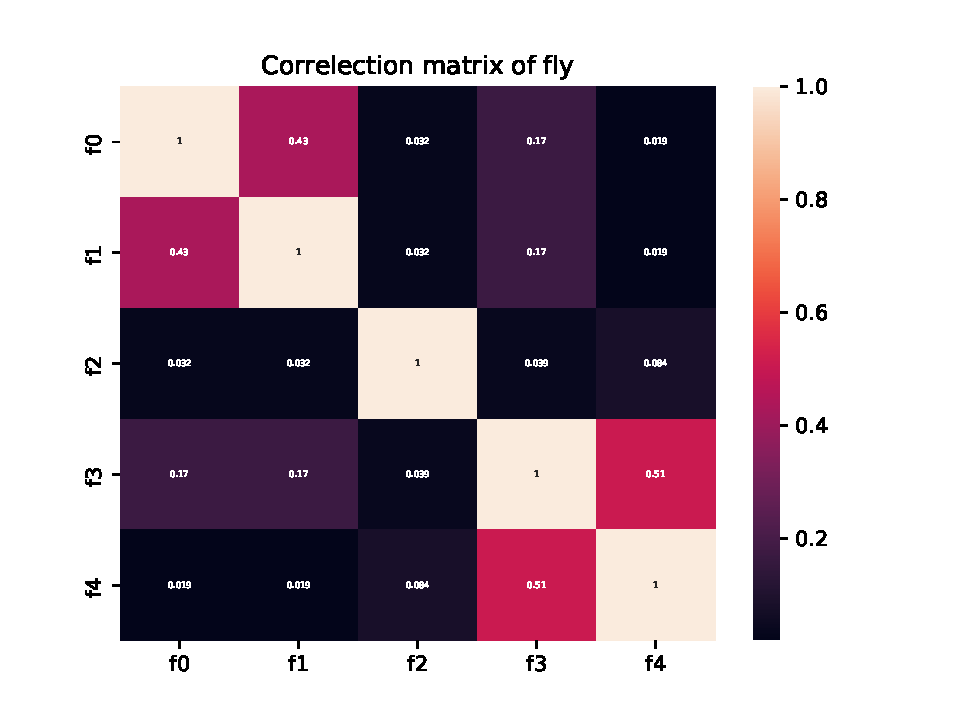
\includegraphics[width=15cm]{Figure/simMatr/fly.pdf}
    \caption{matrici di similarità delle frasi appartenenti al topic travel. Il campione usato per travel è quello che riporta le similarità più basse rispetto a tutti gli altri topic, infatti, il valore di similarità più basso viene registrato dalle coppie [f4, f0] e [f4, f1] che hanno un valore di similarità pari a 0.019. In generale in questo campione la similarità è molto bassa arrivando ad un massimo di 0.51.}
    \label{fig:mtrsim_t}
\end{figure}
\FloatBarrier

\begin{figure}[h!t]
    \centering
    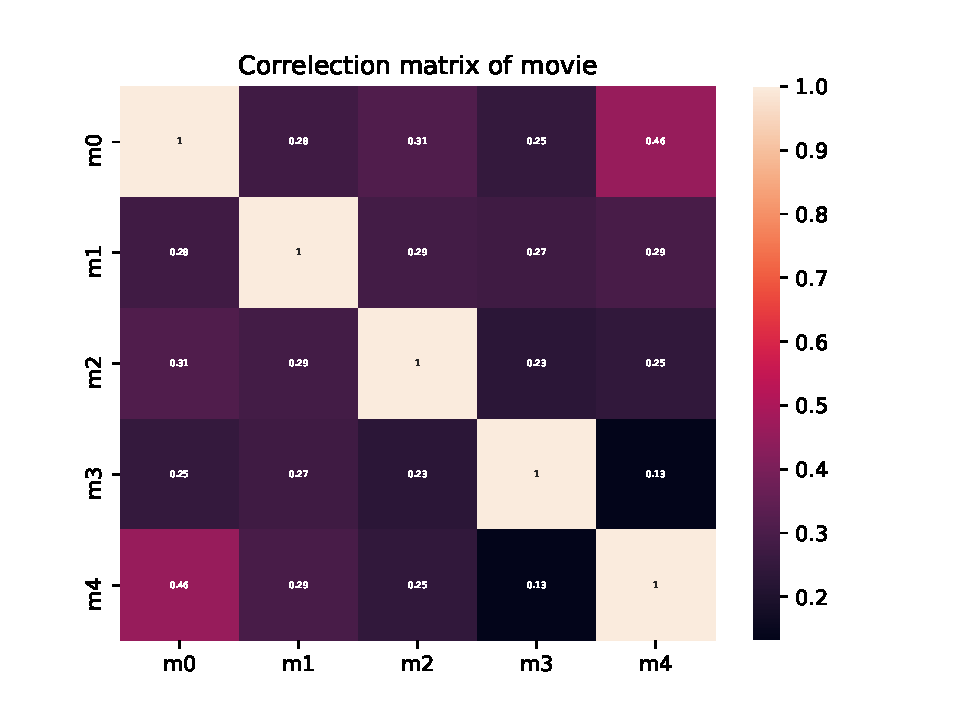
\includegraphics{Figure/simMatr/movie.pdf}
    \caption{matrici di similarità delle frasi appartenenti al topic general. Anche nel topic general si trovano dei valori di similarità molto bassi, ma essi risultano essere comunque migliori dei valori di similarità presenti nel topic travel. I valori di similarità presenti in questo campione vanno da un minimo id 0.13 a un massimo di 0.46.}
    \label{fig:mtrsim_g}
\end{figure}
\FloatBarrier

\begin{figure}[h!t]
    \centering
    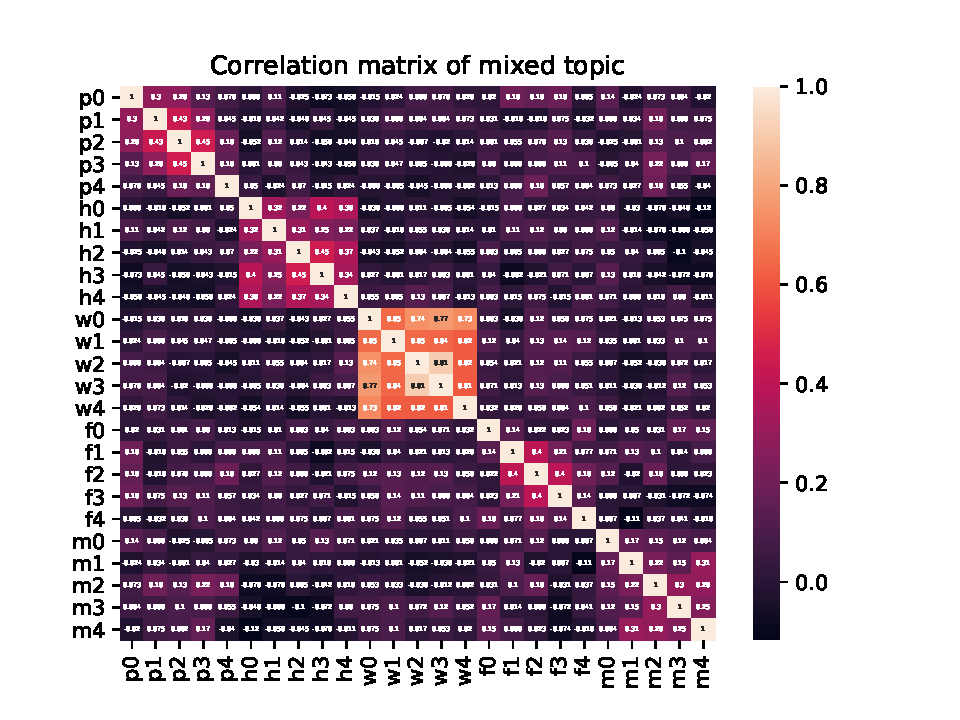
\includegraphics{Figure/simMatr/mixed.pdf}
    \caption{matrici di similarità delle frasi appartenenti ai diversi topic. In questa matrice di confusione sono presenti i valori di similarità ottenuti facendo l'inner product di tutte le frasi appartenenti ai divesi topic. Infatti si può notare che colori delle celle vicine alla diagonale principale sono più chiari dato che le coppie vicino alla diagonale principale sono formate da frasi appartenenti allo stesso topic. Nella parte più esterna della matrice si può osservare che i colori sono più scuri dato che all'esterno della diagonale principale vi sono le coppie di frasi formate da frasi appartenenti a diversi topic. Quindi s può affermare che frasi appartenti allo stesso topic siano più simili fra loro rispetto a frasi che appartengono a topic diversi.}
    \label{fig:mtrsim_mix}
\end{figure}
\FloatBarrier

\subsubsection{Text labeling}
\label{sssec:textlabeling}
Dopo aver rappresentato efficacemente il dataset di testi scritti in linguaggio naturale, si è passati alla fase di labeling, che consiste nell'assegnazione di una classe di appartenenza a ciascun sample. In questo caso, l'operazione è automatica in quanto i sample sono già implicitamente etichettati, in base al dataset da cui provengono. In Tabella~\ref{tbl:mtc} è mostrata la logica di labeling.


\begin{table}[h!t]
\centering
\begin{tabular}{c|c|c}
\toprule
\textbf{Topic} & \textbf{\# sample} & \textbf{Label} \\ \midrule
Politics & 1000 & 0 \\ 
Health & 1000& 1 \\ 
Job & 1000& 2 \\ 
Travel & 1000& 3 \\ 
General & 1000& 4 \\ \bottomrule
\end{tabular}
\caption{Logica di conversione da topic a etichette 
numeriche e informazioni dataset.}
\label{tbl:mtc}
\end{table}

\subsection{Validation}
\label{ssec:validation_Topic}
Inizialmente abbiamo diviso il dataset in Tabella~\ref{tbl:mtc} in un 80\% riservato al training ed un 20\% riservato al testing attraverso la funzione {\tt train\_test\_split} (\textit{stratified}) di scikit-learn\footnote{\url{https://scikit-learn.org/stable/}} per Python.

È stata effettuata una fase di validation sfruttando il training set. In particolare si è adoperata la \textbf{k-fold} cross-validation, una procedura di resampling utilizzata per valutare modelli di machine learning su un campione di dati limitato. La procedura ha come unico parametro \textit{k} che rappresenta il numero di quanti subset si devono creare partendo dal campione originale, nel nostro caso $ k = 5 $.

Tale fase è stata sfruttata anche per l'hyper-parameter tuning usando il metodo {\tt GridSearchCV} di scikit-learn per Python.

In questo lavoro è stato utilizzato uno dei più popolari modelli di machine learning disponibile in letteratura e implementato in scikit-learn, esso è il Random Forest(Sezione~\ref{ssec:RF}). Le sue prestazioni si basano principalmente sul \textit{numero di stimatori}, quindi abbiamo testato da 20 a 1000 stimatori. I migliori risultati sono stati trovati tra 100 e 550 stimatori.

In questa fase si è tentato di massimizzare il parametro F-score (vedi Sezione~\ref{metrics}), impostando oppurtunamente {\tt scoring} di {\tt GridSearchCV}.

\begin{table}[h]
\centering
\begin{tabular}{|c|c|c|}
\hline
\textbf{\# estimatori} & \textbf{Variazione} & \textbf{Risultato} \\ \hline
17 & +/-0.012 & 0.948 \\ \hline
37 & +/-0.010 & 0.963 \\ \hline
51 & +/-0.009 & 0.965 \\ \hline
177 & +/-0.006 & 0.966 \\ \hline
213 & +/-0.006 & 0.968 \\ \hline
517 & +/-0.005 & 0.966 \\ \hline
\end{tabular}
\caption{risultati ottenuti dalla fase di validation}
\label{tab:validationresult}
\end{table}
\FloatBarrier

\subsection{Testing}
\label{ssec:testing_Topic}
Una volta ottenuti i migliori parametri per ciascun classificatore abbiamo valutato le loro performance sul dataset di testing.

La tabella~\ref{tbl:training_ds1000} riporta le performance ottenute da ciascun classificatore sul testing set.
\begin{table}[h]
\begin{tabular}{|l|l|c|c|c|c|c|}
\hline
\multirow{2}{*}{\textbf{Classifier}} & \multirow{2}{*}{\textbf{Metric}} & \multicolumn{5}{c|}{\textbf{Topics}} \\ \cline{3-7} 
 &  & Politics & Health & Job & Travel & General \\ \hline
\multirow{4}{*}{RF} & Accuracy & \multicolumn{5}{c|}{0.983} \\ \cline{2-7} 
 & Precision & 0.979 & 0.99 & 0.985 & 0.966 & 0.994 \\ \cline{2-7} 
 & Recall & 0.965 & 0.995 & 0.985  & 0.995 & 0.975 \\ \cline{2-7} 
 & Fscore & 0.972 & 0.992 & 0.985 & 0.980 & 0.984 \\ \hline
\end{tabular}
\caption{Risultati per la fase di testing di Random Forest sul dataset ds1000.csv}
\label{tbl:training_ds1000}
\end{table}
\FloatBarrier
Si ricorda che l'obiettivo di questo step è di sviluppare un metodo per riconoscere il topic d'appartenenza di un testo scritto in linguaggio naturale con riferimento ai quattro topic più citati nella letteratura sulla privacy\cite{looseTweets,dontTweetThis}, più un topic generico. In particolare, si vuole avere un classificatore capace di ottenere buone prestazioni su tutte le classi individuate. 

Il \textit{TopicClassifier} basato su RF\ref{ssec:RF} così addestrato è stato \quotes{dumpato} in un oggetto {\tt pickle}\footnote{https://docs.python.org/3/library/pickle.html}.

\subsection{Testing \textit{into the wild}}
\label{ssec:testing_wild}
\textit{TopicClassifier} è stato oggetto di una ulteriore fase di testing. Si è pensato di misurare le performance del classificatore su un dataset molto più ampio, rinominato \quotes{wild dataset}. Wild dataset è composto da 2000 elementi per ciascun topic/categoria (politics, health, job, travel e general) non appartenenti al dataset di addestramento nè a quello di testing precedentemente visto.

La tabella~\ref{tbl:testing_wild} riporta le misure ottenute dalla sperimentazione \textit{into the wild} di \textit{TopicClassifier}. 
\begin{table}[h]
\begin{tabular}{|l|l|c|c|c|c|c|}
\hline
\multirow{2}{*}{\textbf{Classifier}} & \multirow{2}{*}{\textbf{Metric}} & \multicolumn{5}{c|}{\textbf{Topics}} \\ \cline{3-7} 
 &  & Politics & Health & Job & Travel & General \\ \hline
\multirow{4}{*}{RF} & Accuracy & \multicolumn{5}{c|}{0.988} \\ \cline{2-7} 
 & Precision & 0.992 & 0.995 & 0.985 & 0.975 & 0.993 \\ \cline{2-7} 
 & Recall & 0.969 & 0.995 & 0.993 & 0.996 & 0.988 \\ \cline{2-7} 
 & Fscore & 0.980 & 0.995 & 0.989 & 0.985 & 0.999 \\ \hline
\end{tabular}
\caption{Risultati della fase di testing sul dataset wild}
\label{tbl:testing_wild}
\end{table}
\FloatBarrier
\textit{TopicClassifier} durante l'esperimento \textit{into the wild} mostra delle performace simili a quelle ottenute durante la fase di testing (Sezione~\ref{ssec:testing_Topic}), ragion per cui si può affermare di aver effettuato una fase di training efficace.

\section{Sensitivity classification}
\label{sec:sensclass}
Una volta ottenuto un classificatore in grado di riconoscere il topic d'appartenenza di un testo scritto in linguaggio naturale con riferimento ai quattro topic più citati nella letteratura sulla privacy, più un topic generico, il focus si sposta sul capire se una data frase (appartente ad un topic specifico) contenga o meno dati sensibili e/o personali. Un esempio di testo con contenuti sensibili e non sensibili è riportato in Tabella~\ref{tbl:example_sens}.

\begin{table}[h]

\centering
\begin{tabular}{c|c|c}
\hline
\textbf{Frase} & \textbf{Topic} & \textbf{Sensibile} \\ \hline
\textit{Questa notte non ho dormito} & Health & \textbf{No} \\ \hline
\textit{Soffro di insonnia} & Health & \textbf{Sì} \\ \hline
\end{tabular}
\caption{esempio di contenuti sensibili e non}
\label{tbl:example_sens}
\end{table}
\FloatBarrier

A tal fine, è stata definita una metodologia come segue (vedi Figura~\ref{fig:methodsens}):
\begin{itemize}
    \item Creazione Dataset sensitivity (Sezione~\ref{ssec:create_sens_ds}): rappresentazione dei sample e labeling dei dati;
    \item Validation: validazione del modello realizzato usando la k-fold cross-validation;
    \item Testing: testing delle performance del metodo sul test set.
\end{itemize}

\begin{figure}[h!t]
    \centering
    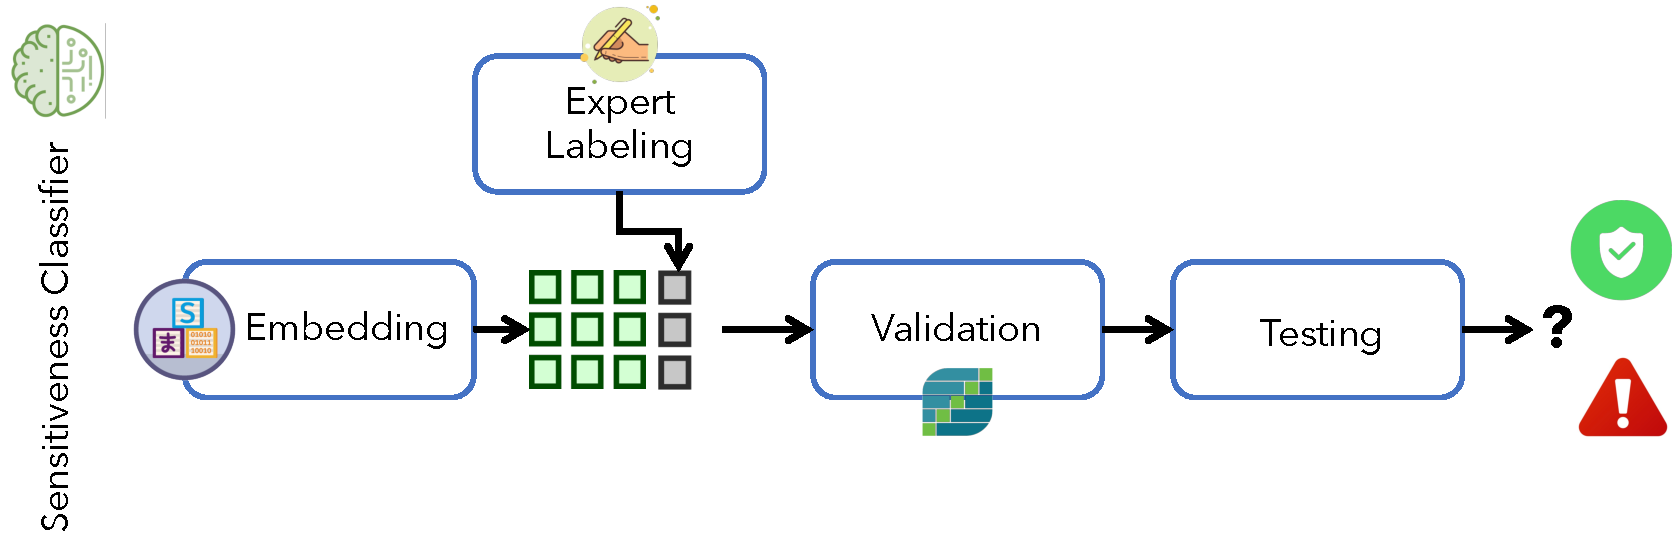
\includegraphics[width=15cm]{Figure/grafici/sensitivenessmethod_cropped.pdf}
    \caption{Principali fasi per la creazione del modulo Sensitiveness classifier: (\textit{Embedding}) le frasi dei vari dataset vengono trasformate in vettori a lunghezza fissa; (\textit{Expert labeling}) tramite una serie di regole ben definite~\cite{}, un esperto del dominio effettua manualmente il labeling dei sample; (\textit{Validation}) mediante una k-fold cross-validation si validano vari classificatori basati sul supervised learning e si effettua il tuning degli iper-parametri utilizzando il training set $trs'$; (\textit{Testing}) una volta ottenuti i migliori parametri per ciascun classificatore, si effettua il testing sul test set $tss'$;   }
    \label{fig:methodsens}
\end{figure}

\subsection{Creazione Dataset sensitivity}
\label{ssec:create_sens_ds}
Per la creazione di questo dataset abbiamo riutilizzato parte del {\tt ds1000.csv} precedentemente creato per la fase di Topic Classification~\ref{tbl:training_ds1000}. In particolare abbiamo selezionato con una funzione {\tt random} 200 elementi per ciascuna categoria di riferimento.

\begin{table}[h!t]
    \centering
    \begin{tabular}{c|c|c}
    \hline
        \textbf{Topic} & \textbf{ID} & \textbf{\# entry} \\ \hline
        Politics & 0 & 200 \\ \hline
        Health & 1 & 200 \\ \hline
        Job & 2 & 200 \\ \hline
        Travel & 3 & 200 \\ \hline
        General & 4 & 200 \\ \hline
    \end{tabular}
    \caption{ds200.csv, il dataset da 200 elementi per topic}
    \label{tab:ds200.csv}
\end{table}
\FloatBarrier

\subsubsection{Sensitiveness labeling}
\label{sssec:sens_labeling}
In questa fase ds200.csv è stato etichettato secondo le regole delineate in~\cite{dataSpectrum}.
\begin{figure}
    \centering
    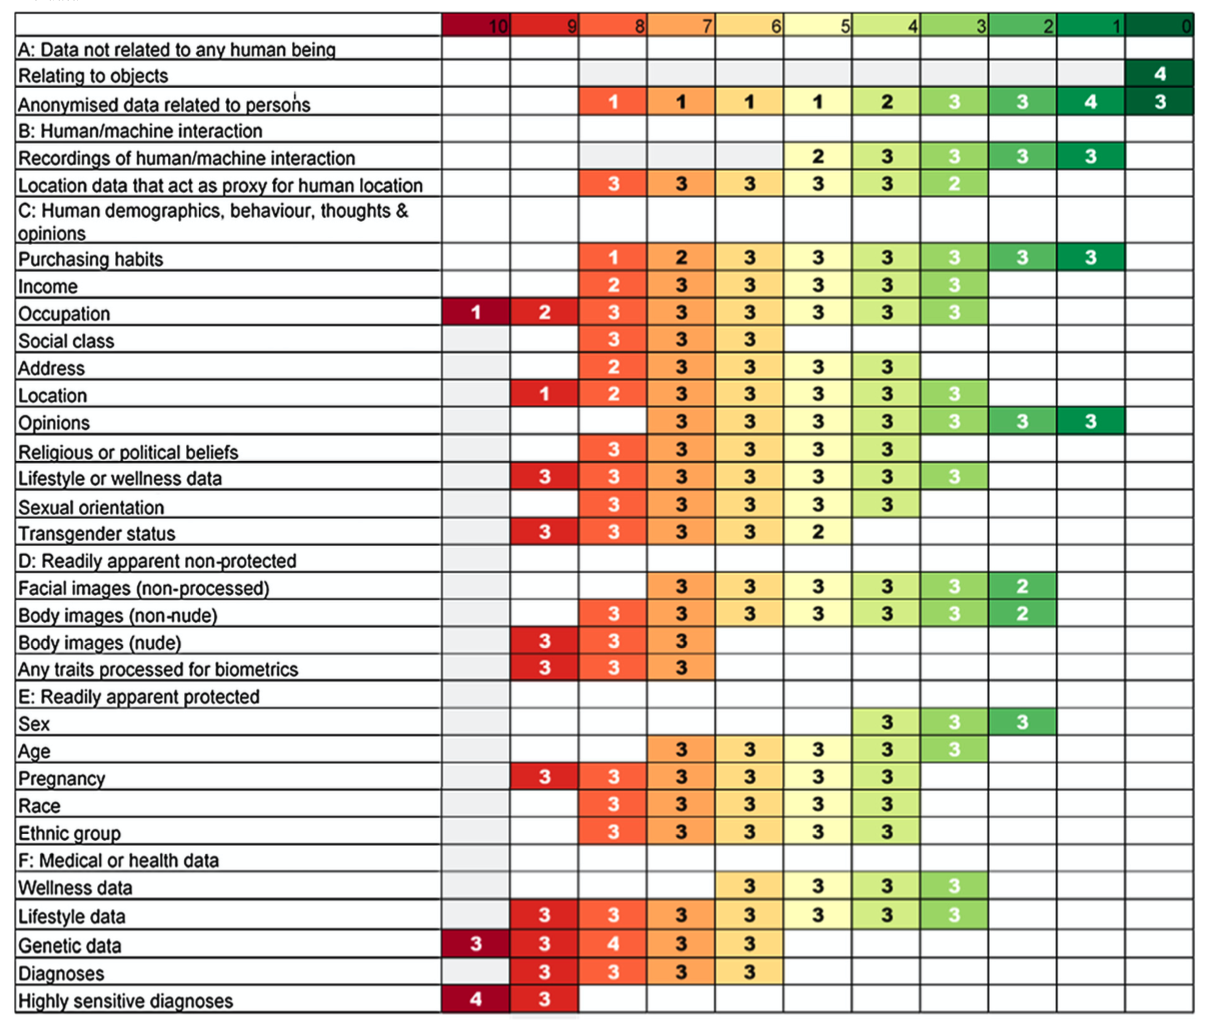
\includegraphics[scale=0.4]{Figure/sensTbl.png}
    \caption{Tabella delle sensibilità utilizzata da Rumbold et al.~\cite{dataSpectrum}}
    \label{fig:sensRumboldd}
\end{figure}
\FloatBarrier
Le righe della tabella mostrate in figura~\ref{fig:sensRumboldd} contengono la categoria a cui una frase può appartenere e quanto essa possa essere sensibile, il \textbf{livello di sensibilità} varia da 0 (non sensibile) a 10 (molto sensibile). I numeri presenti nelle celle variano da 0 a 4 ed essi rappresentano la \textbf{frequenza} che l'argomento descritto nella riga si presenti con il livello di sensibilità descritto nella colonna. Ad esempio prendiamo l'argomento \textit{Relating to object} esso ha un livello di sensibilità pari a 0 e nella cella viene riportato il numero 4, questo vuol dire che quando si parlerà di argomenti relativo ad oggetti questi saranno sicuramente poco sensibili.


%\subsubsection{Tabella delle sensibilità}
%\label{ssec:tblSens&Euricstic}
In accordo allo studio fatto da Rumbold et al.~\cite{dataSpectrum} è stata definita una tabella delle sensibilità a cui fare riferimento per determinare se un contenuto va etichettato come sensibile (1) o meno (0). I criteri definiti nella tabella~\ref{tbl:senstbl} sono stati ottenuti utilizzando il seguente metodo.

Si definiscono $freq$ i valori di frequenza utilizzati da Rumbold et al. Sia $freq[i]$ il valore di frequenza per il livello di sensibilità $i$, $i\in[0..10]$.

I livelli $i<5$ indicano basso grado di sensibilità, viceversa i livelli $i>=5$ indicano alto grado di sensibilità. 

Calcoliamo quindi lo score totale di sensibilità come

$\sum^{N}_{i=x}freq[i]$, $N=4,10$, $x=0,5$. 

Etichettiamo un elemento non sensibile se:
\begin{equation}
\sum^{4}_{i=0}freq[i] > \sum^{10}_{i=5}freq[i]
\end{equation}

Viceversa, se sensibile.

Informalmente, si confronta la somma delle frequenze che hanno un livello di sensibilità compreso fra $0$ e $4$ con la somma delle frequenze che hanno un livello di sensibilità compreso fra $5$ e $10$. Se la somma delle frequenze che hanno un livello di sensibilità compreso fra $5$ e $10$ è maggiore rispetto alla somma delle frequenze che hanno un livello di sensibilità compreso fra $0$ e $4$ allora l'argomento risulta essere sensibile e i testi che appartengono a tale argomento verranno etichettati con $1$, $0$ altrimenti.

\begin{table}[h]
\centering 
\begin{tabular}{|l|c|}
\hline
\multicolumn{1}{|c|}{\textbf{Regole}} & \textbf{Sensibile} \\ \hline
Dati relativi ad oggetti & \xmark \\ \hline
Dati anonimizzati relativi a persone & \xmark \\ \hline
Dati relativi ad interazioni uomo-macchina & \xmark \\\hline
Dati relativi a posizione di uomini & \cmark \\ \hline
Dati relativi ad abitudini di acquisto & \xmark \\\hline
Dati relativi allo stipendio & \cmark \\ \hline
Dati relativi al lavoro svolto & \cmark \\ \hline
Dati relativi alla propria classe sociale & \cmark \\ \hline
Indirizzo o luogo & \cmark \\ \hline
Chiara opinione religiosa o politica & \cmark \\ \hline
Altri tipi di opinioni & \xmark \\\hline
Dati sul lifestyle & \cmark \\ \hline
Orientamento sessuale & \cmark \\ \hline
Sesso in generale & \xmark \\ \hline
Dati relativi alla gravidanza & \cmark \\ \hline
Dati relativi al gruppo etnico & \cmark \\ \hline
Dati medici o stato di salute & \cmark \\ \hline
\end{tabular}
\caption{Regole per effettuare il labeling manuale. \cmark indica che una frase contenente quel dato è sensibile, \xmark viceversa.}
\label{tbl:senstbl}
\end{table}
\FloatBarrier

Una volta completata l'etichettatura abbiamo ottenuto un certo numero di testi sensibili per ogni topic. I principali dati di riferimento per questo dataset sono riportati nella tabella~\ref{tbl:ds200}.

\begin{table}[h]
\centering
\begin{tabular}{|c|c|c|}
\hline
\textbf{Topic} & \textbf{\# entry} & \textbf{\# entry sensibili} \\ \hline
Politics & 200 & 100 \\ \hline
Health & 200 & 100 \\ \hline
Job & 200 & 80 \\ \hline
Travel & 200 & 100 \\ \hline
General & 200 & 100 \\ \hline
Totale & 1000 & 480 \\ \hline
\end{tabular}
\caption{ds200.csv}
\label{tbl:ds200}
\end{table}
\FloatBarrier

\subsection{Approcci per l'analisi di sensitività}
\label{ssec:approcci}
Per analizzare il livello di sensitività di una frase abbiamo individuato due possibili tecniche mostrate in figura~\ref{fig:approccisens}:
\begin{enumerate}
    \item realizzare un singolo classificatore che è addestrato per riconoscere ed individuare se una frase contiene dati sensibili/personali o meno sull'intero dataset {\tt ds200.csv};
    \item realizzare 5 classificatori diversi, uno per ciascun topic, capaci di riconoscere ed individuare se una frase che parla di un certo argomento (cioè che appartiene ad uno dei topic di cui alla Sezione~\ref{sssec:multiclass}) contiene dati sensibili/personali o meno.
\end{enumerate}
Date le buone performance mostrate dalla classificazione per topic effettuata con il Random Forest (Sezione~\ref{sec:topicclass}), si è scelto di utilizzare Random Forest in entrambi gli approcci.

\begin{figure}[h]
    \centering
    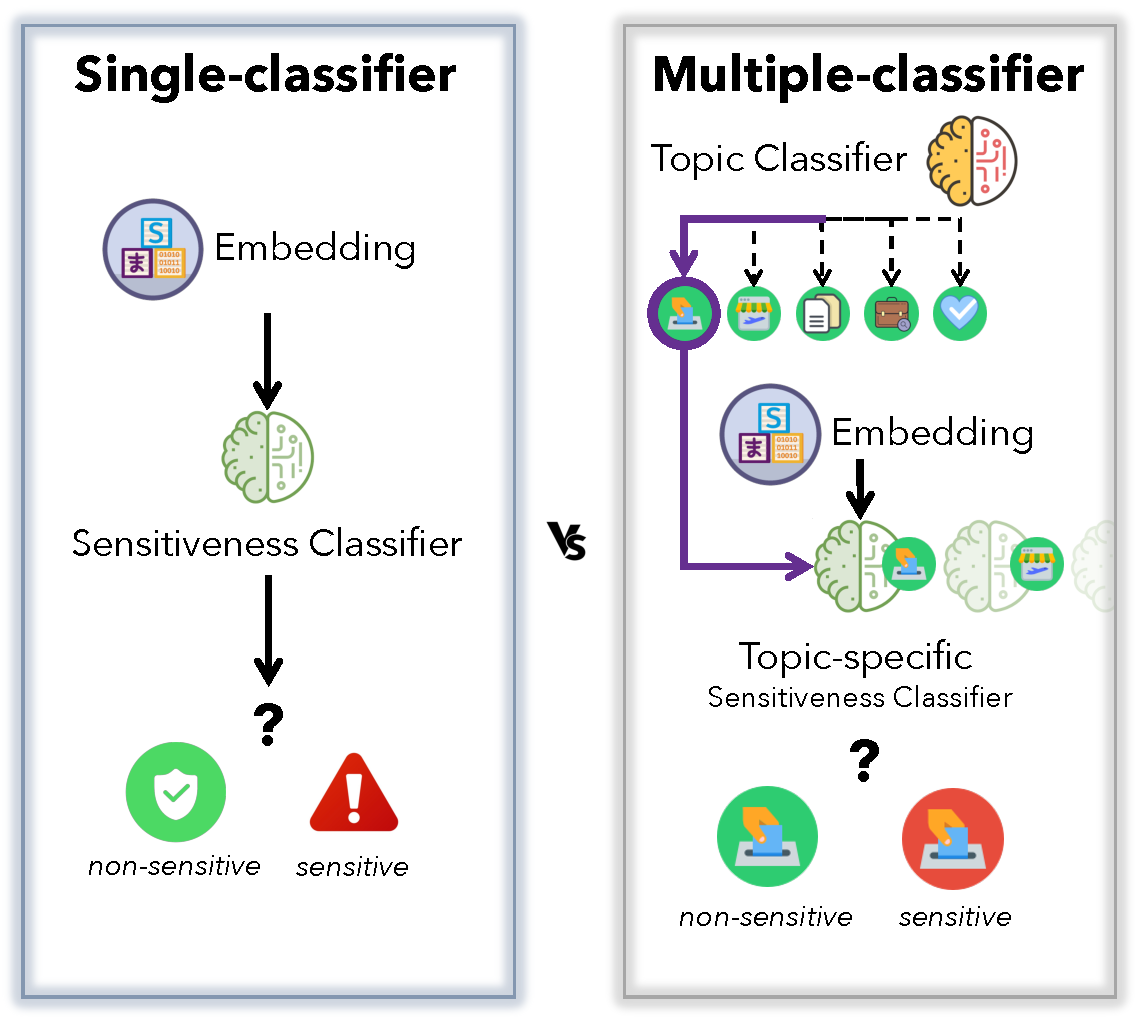
\includegraphics[width=15cm]{Figure/grafici/vs_cropped.pdf}
    \caption{I due approcci per la creazione del Sensitiveness classifier.}
    \label{fig:approccisens}
\end{figure}
\FloatBarrier



\subsubsection{Approccio con il singolo classificatore}
\label{sssec:singleclass}
Con questo approccio viene realizzato un singolo classificatore in grado di riconosce frasi contenenti dati sensibili e/o personali. Il vantaggio è quello di avere un unico classificatore sensitività in grado di individuare contenuti sensibili, lo svantaggio è il fatto che questo tipo di classificatore ha una conoscenza a grana grossa della di un dato sensibile e quindi è facile che sbagli ad assegnare il grado di sensibilità.

\paragraph{Validation} Il dataset è stato diviso in 80\% per il training e 20\% per il testing con la funzione {\tt train\_test\_split}. Il dataset di training è oggetto della validation. Abbiamo effettuato una k-fold cross-validation con $k=10$ utilizzando il metodo {\tt GridSearchCV} di scikit-learn per Python cercando di ottimizzare il roc\_auc score. In Tabella~\ref{tbl:validation_sens} si mostrano sia i parametri oggetto della funzione {\tt GridSearchCV} sia i risultati raggiunti in termini di roc\_auc score. 
\begin{table}[h]
\centering
\begin{tabular}{|c|c|c|}
\hline
\textbf{Estimatori} & \textbf{Variazione} & \textbf{Roc-AUC} \\ \hline
17 & +/-0.061 & 0.760 \\ \hline
37 & +/-0.079 & 0.783 \\ \hline
51 & +/-0.075 & 0.806 \\ \hline
177 & +/-0.076 & 0.836 \\ \hline
213 & +/-0.041 & 0.840 \\ \hline
517 & +/-0.057 & 0.847 \\ \hline
1013 & +/-0.058 & 0.851 \\ \hline
\end{tabular}
\caption{ROC AUC score ottenuti in fase di validation con Random Forest nel caso single-classifier.}
\label{tbl:validation_sens}
\end{table}
\FloatBarrier

\paragraph{Testing} Dopo la fase di validazione, sono stati ottenuti i migliori parametri per il classificatore Random Forest. Il modello viene quindi ri-addestrato sul training set e se ne misurano le performance sul test set. I risulati sono riportati in Tabella~\ref{tbl:training_sens}.

\begin{table}[h]

\centering
\begin{tabular}{|c|c|c|}
\hline
\textbf{Metric} & \textbf{Non Sensibile} & \textbf{Sensibile} \\ \hline
Accuracy & \multicolumn{2}{c|}{0.765} \\ \hline
Precision & 0.776 & 0.752 \\ \hline
Recall & 0.769 & 0.760 \\ \hline
Roc-Auc & \multicolumn{2}{c|}{0.848} \\ \hline
\end{tabular}
\caption{Performance del classificatore Random Forest ottenute nella fase di testing con approccio single-classifier.}
\label{tbl:training_sens}
\end{table}
\FloatBarrier

Matrice di confusione per questo test è mostrata in Figura~\ref{fig:mtrconf_sim_200}.


Tenuto conto della difficoltà di questo task, le performance del classificatore di sensibilità singolo sono discrete.

\subsubsection{Approccio con classificatori multipli}
\label{sssec:multiclass}
L'altro approccio al problema della sensibilità di un testo è quello di avere cinque classificatori differenti (uno per ogni topic) che verranno addestrati a riconoscere argomenti sensibili sui 200 elementi che appartengono ad ogni topic di {\tt ds200.csv}.

Di seguito sono mostrati tutti i risultati ottenuti durante la validation e il testing dei vari classificatori di sensibilità. Per esigenze di spazio, e leggibilità del documento, le matrici di confusione di ogni classificatore nella fase di testing sono state riportate in Appendice~(\ref{ch:appendix}).

\subsubsection{Validation e testing sensitiveness politics}
\label{sssec:val_testing_pol}
\paragraph{Validation} La fase di validation per ciascuno dei classificatori di sensibilità è la medesima: si suddivide il dataset in 80\% per training e 20\% per testing con la funzione {\tt train\_test\_split} di scikit-learn per Python. Il dataset di training è oggetto della validazione vera e propria che avviene con il metodo {\tt GridSearchCV} in cui si testano diversi parametri per il classificatore e si tenta di ottimizzare il roc\_auc score.  I risultati di questa fase sono riportati nelle Tabelle~\cref{tbl:val_sens_pol,tbl:val_sens_health,tbl:val_sens_travel,tbl:val_sens_job,tbl:val_sens_general}, per i topic Politica, Salute, Viaggi, Lavoro e General rispettivamente.

\paragraph{Testing} Una volta ottenuti i migliori parametri per il classificatore, il modello viene ri-addestrato sul training set e se ne misurano le performance sul test set.  I risultati di questa fase sono riportati nelle Tabelle~\cref{tbl:training_sens_pol,tbl:training_sens_health,tbl:training_sens_travel,tbl:training_sens_job,tbl:training_sens_general}, per i topic Politica, Salute, Viaggi, Lavoro e General rispettivamente.


\begin{table}[h]

\centering
\begin{tabular}{|c|c|c|}
\hline
\textbf{Estimator} & \textbf{Variazione} & \textbf{Roc-AUC} \\ \hline
17 & +/-0.240 & 0.781 \\ \hline
37 & +/-0.118 & 0.858 \\ \hline
51 & +/-0.209 & 0.858 \\ \hline
177 & +/-0.122 & 0.888 \\ \hline
213 & +/-0.181 & 0.878 \\ \hline
517 & +/-0.143 & 0.890 \\ \hline
1013 & +/-0.146 & 0.884 \\ \hline
\end{tabular}
\caption{Risultati della validation per il classificatore di sensitivà \textit{politica}}
\label{tbl:val_sens_pol}
\end{table}
\FloatBarrier

\begin{table}[h]
\centering
\begin{tabular}{|c|c|c|}
\hline
\textbf{Metric} & \textbf{Non Sensibile} & \textbf{Sensibile} \\ \hline
Accuracy & \multicolumn{2}{c|}{0.765} \\ \hline
Precision & 0.695 & 0.764 \\ \hline
Recall & 0.8 & 0.65 \\ \hline
Roc-Auc & \multicolumn{2}{c|}{0.773} \\ \hline
\end{tabular}
\caption{risultati del testing per classificatore di sensitivà \textit{politica}}
\label{tbl:training_sens_pol}
\end{table}
\FloatBarrier

%Matrice di confusione~\ref{fig:mtrconf_sim_p}

\subsubsection{Validation e testing sensitiveness health}
\label{sssec:val_testing_health}

\begin{table}[h]

\centering
\begin{tabular}{|c|c|c|}
\hline
\textbf{Estimator} & \textbf{Variazione} & \textbf{Roc-AUC} \\ \hline
17 & +/-0.095 & 0.945 \\ \hline
37 & +/-0.062 & 0.963 \\ \hline
51 & +/-0.092 & 0.956 \\ \hline
177 & +/-0.101 & 0.952 \\ \hline
213 & +/-0.059 & 0.964 \\ \hline
517 & +/-0.086 & 0.958 \\ \hline
1013 & +/-0.073 & 0.961 \\ \hline
\end{tabular}
\caption{Risultati della validation per classificatore di sensitivà \textit{health}}
\label{tbl:val_sens_health}
\end{table}
\FloatBarrier

\begin{table}[h]

\centering
\begin{tabular}{|c|c|c|}
\hline
\textbf{Metric} & \textbf{Non Sensibile} & \textbf{Sensibile} \\ \hline
Accuracy & \multicolumn{2}{c|}{0.875} \\ \hline
Precision & 0.894 & 0.857 \\ \hline
Recall & 0.85 & 0.9 \\ \hline
Roc-Auc & \multicolumn{2}{c|}{0.935} \\ \hline
\end{tabular}
\caption{Risultati del testing per il classificatore di sensitivà \textit{health}}
\label{tbl:training_sens_health}
\end{table}
\FloatBarrier

%Matrice di confusione~\ref{fig:mtrconf_sim_h}

\subsubsection{Validation e testing sensitiveness job}
\label{sssec:val_testing_job}

\begin{table}[h]

\centering
\begin{tabular}{|c|c|c|}
\hline
\textbf{Estimator} & \textbf{Variazione} & \textbf{Roc-AUC} \\ \hline
17 & +/-0.191 & 0.893 \\ \hline
37 & +/-0.123 & 0.873 \\ \hline
51 & +/-0.150 & 0.884 \\ \hline
177 & +/-0.150 & 0.894 \\ \hline
213 & +/-0.115 & 0.908 \\ \hline
517 & +/-0.111 & 0.908 \\ \hline
1013 & +/-0.119 & 0.914 \\ \hline
\end{tabular}
\caption{Risultati della validation per il classificatore di sensitivà \textit{job}}
\label{tbl:val_sens_job}
\end{table}
\FloatBarrier

\begin{table}[h]

\centering
\begin{tabular}{|c|c|c|}
\hline
\textbf{Metric} & \textbf{Non Sensibile} & \textbf{Sensibile} \\ \hline
Accuracy & \multicolumn{2}{c|}{0.85} \\ \hline
Precision & 0.814 & 0.923 \\ \hline
Recall & 0.956 & 0.705 \\ \hline
Roc-Auc & \multicolumn{2}{c|}{0.928} \\ \hline
\end{tabular}
\caption{Risultati del testing per il classificatore di sensitivà \textit{job}}
\label{tbl:training_sens_job}
\end{table}
\FloatBarrier

%Matrice di confusione~\ref{fig:mtrconf_sim_j}

\subsubsection{Validation e testing sensitiveness travel}
\label{sssec:val_testing_travel}

\begin{table}[h]

\centering
\begin{tabular}{|c|c|c|}
\hline
\textbf{Estimator} & \textbf{Variazione} & \textbf{Roc-AUC} \\ \hline
17 & +/-0.225 & 0.835 \\ \hline
37 & +/-0.136 & 0.878 \\ \hline
51 & +/-0.153 & 0.883 \\ \hline
177 & +/-0.117 & 0.903 \\ \hline
213 & +/-0.114 & 0.894 \\ \hline
517 & +/-0.098 & 0.905 \\ \hline
1013 & +/-0.092 & 0.903 \\ \hline
\end{tabular}
\caption{Risultati della validation per il classificatore di sensitivà travel}
\label{tbl:val_sens_travel}
\end{table}
\FloatBarrier

\begin{table}[h]

\centering
\begin{tabular}{|c|c|c|}
\hline
\textbf{Metric} & \textbf{Non Sensibile} & \textbf{Sensibile} \\ \hline
Accuracy & \multicolumn{2}{c|}{0.85} \\ \hline
Precision & 0.791 & 0.937 \\ \hline
Recall & 0.95 & 0.75 \\ \hline
Roc-Auc & \multicolumn{2}{c|}{0.971} \\ \hline
\end{tabular}
\caption{risultati del testing per il classificatore di sensitivà \textit{travel}}
\label{tbl:training_sens_travel}
\end{table}
\FloatBarrier

%Matrice di confusione~\ref{fig:mtrconf_sim_t}

\subsubsection{Validation e testing sensitiveness general}
\label{sssec:val_testing_general}

\begin{table}[h]

\centering
\begin{tabular}{|c|c|c|}
\hline
\textbf{Estimator} & \textbf{Variazione} & \textbf{Roc-AUC} \\ \hline
17 & +/-0.251 & 0.552 \\ \hline
37 & +/-0.189 & 0.578 \\ \hline
51 & +/-0.182 & 0.590 \\ \hline
177 & +/-0.232 & 0.656 \\ \hline
213 & +/-0.221 & 0.597 \\ \hline
517 & +/-0.233 & 0.656 \\ \hline
1013 & +/-0.189 & 0.637 \\ \hline
\end{tabular}
\caption{Risultati della validation per il classificatore di sensitivà \textit{general}}
\label{tbl:val_sens_general}
\end{table}
\FloatBarrier

\begin{table}[h]

\centering
\begin{tabular}{|c|c|c|}
\hline
\textbf{Metric} & \textbf{Non Sensibile} & \textbf{Sensibile} \\ \hline
Accuracy & \multicolumn{2}{c|}{0.6} \\ \hline
Precision & 0.593 & 0.625 \\ \hline
Recall & 0.863 & 0.277 \\ \hline
Roc-Auc & \multicolumn{2}{c|}{0.736} \\ \hline
\end{tabular}
\caption{Risultati del testing per classificatore di sensitivà general}
\label{tbl:training_sens_general}
\end{table}
\FloatBarrier

%Matrice di confusione~\ref{fig:mtrconf_sim_g}

Dai risultati ottenuti si evince che i classificatori di sensibilità multipli (tranne nel caso di general) sono più accurati o comparabili rispetto al singolo classificatore di sensibilità. Dunque, consapevoli del fatto le performance del classificatore di sensibilità general vanno migliorate si è deciso di adottare la soluzione con 5 classificatori di sensibilità. In ottica di implementazione di un tool completo, ad un punteggio di Technology Readiness Level (TRL) alto, è preferibile avere diversi classificatori addestrati per un task \quotes{più piccolo}.

\section{Customized sensitivity classification}
\label{sec:pres_sens_class}
La privacy è una percezione soggettiva, in cui ogni utente ha il proprio livello di riservatezza con riguardo alle proprie informazioni private. Ancora più importante, l'atteggiamento verso la privacy varia da un argomento all'altro. 

Ne deriva che la realizzazione di uno sistema che non tenga conto delle esigenze e preferenze degli utenti può risultare in uno strumento ostruente, fastidioso o addirittura inutile. Ragion per cui bisogna sviluppare uno strumento che in qualche modo si adatti alle esigenze e preferenze degli utenti. 

Per effettuare questa operazione esistono diverse tecniche ad esempio Q-learning~\cite{q-learning} e vari tipi di reinforcement learning~\cite{reinforce-learn}, agenti basati su LSTM Network~\cite{lstm}, e così via. Essi sono dei modelli che apprendono sulla base dei feedback ricevuti dall'ambiente in cui sono in esecuzione: ad esempio, il feedback di un utente è utile ad addestrare sistemi di recommendation.

Per catturare l'atteggiamento degli utenti verso la privacy personale, è stato realizzato un modello \textit{online} di learning che in base alla percezione di sensibilità dell'utente sarà in grado di segnalare solo i contenuti che per quel singolo utente risultano sensibili.
A tale scopo ci siamo ispirati al sistema di priority inbox di gmail~\cite{inbox}.
Il sistema è in grado di capire quali mail secondo un utente hanno una priorità maggiore rispetto alle altre. Per realizzarlo, gli autori si sono basati sulle interazioni che gli utenti avevano con le mail in arrivo: ad esempio se una mail veniva aperta dopo più di sette giorni, allora non era una mail importante quindi a quella mail dovrebbe esser assegnata una bassa priorità.

Facendo un opportuno parallelismo, questo scenario risulta abbastanza simile al nostro caso, in quanto l'utente, interagendo con il modello online, dovrebbe fornire feedback riguardo la sua personale percezione di privacy.

\subsection{Realizzazione}
L'intezione è realizzare un modello IA-based lato client in grado di capire il livello di sensibilità dell'utente. La scelta di realizzare questa è IA lato client è obbligata dal momento che un tool per la prevenzione della privacy non deve violare la privacy per prevenirla. Per questo non può essere effettuata una classificazione lato server che comporterebbe privacy leakage verso first-part. Questo vincolo ci porta a dover realizzare un modello che sia \textit{leggero} in maniera tale che non rallenti la normale navigazione dell'utente sul web, e \textit{semplice} da implementare in \textit{JavaScript}. È stato scelto il Passive-Aggressive online learning method~\cite{PAalgo}. Come funziona?

Supponiamo avere un dataset $D$

$$D=\left\{
                \begin{array}{ll}
                  X=\{x_1,x_2,\dots ,x_t,\dots \}, x_i \in \mathbb{R}^n \\
                  Y=\{y_1,y_2,\dots ,y_t,\dots\}, y_i \in \{-1,+1\}
                \end{array}
              \right.$$

L'indice $t$ è stato scelto per contrassegnare la dimensione temporale del problema. In questo caso, infatti, i campioni possono continuare ad arrivare per un tempo indefinito. Naturalmente, se sono tratti dalla stessa distribuzione generatrice di dati, l'algoritmo continuerà ad apprendere (probabilmente senza grandi modifiche ai parametri), ma se sono estratti da una distribuzione completamente diversa, i pesi verranno \quotes{dimenticati} lentamente a favore della nuova distribuzione. Nel nostro caso siamo su un problema di classificazione binaria (-1 dato non sensibile, 1 dato sensibile).

Dato un vettore di peso $w$, la previsione si ottiene semplicemente come:

$$\tilde{y_t}=sign(w^T\cdot x_t)$$

Questo algoritmo si basa sulla Hinge-loss function (la stessa utilizzata da SVM):

$$L(\tilde{\theta})=max(0,1-y\cdot f(x_t,\theta))$$

Il valore di $L$ è limitato tra $0$ (che significa corrispondenza perfetta) e $K$ a seconda di $f(x(t), \theta)$ con $K > 0$ (previsione completamente errata). Un algoritmo Passive-Aggressive funziona genericamente con questa regola di aggiornamento:

$$\left\{
                \begin{array}{ll}
                  w_{t+1}=argmin_w\frac{1}{2}\| w-w_t\|^2 +C\xi^2\\
                  L(w;x_t;y_t) < \xi
                \end{array}
              \right.$$
              
Per comprendere questa regola, supponiamo che la variabile di gioco $\xi = 0$ (e $L$ vincolata a $0$). Se viene presentato un campione $x(t)$, il classificatore utilizza il vettore di peso corrente per determinare il segno. Se il segno è corretto, la funzione loss è $0$ e l'argmin è $w(t)$. Ciò significa che l'algoritmo è passivo quando si verifica una classificazione corretta. Supponiamo ora che si sia verificata un'errata classificazione (vedi Figura~\ref{fig:PAII1}).            
              
\begin{figure}[h]
    \centering
    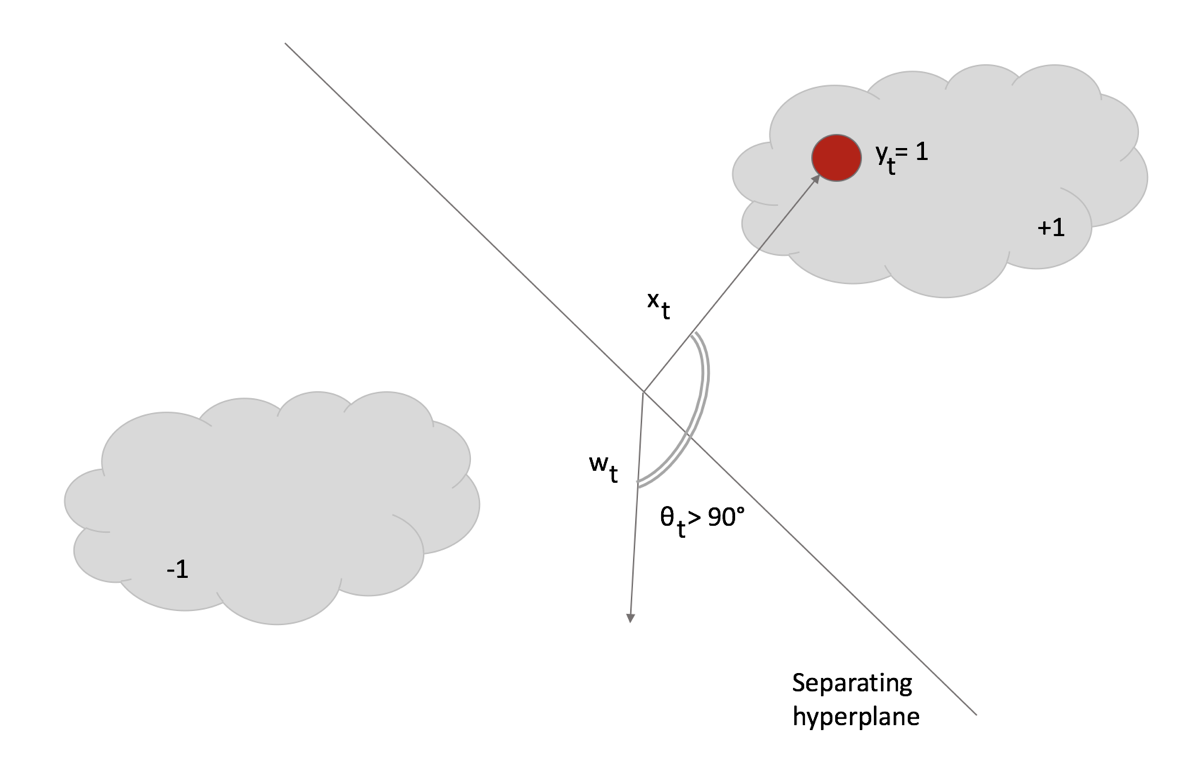
\includegraphics[scale=0.5]{Figure/PAII1.png}
    \caption{Iperpiano e vettore $w$, in fase passiva}
    \label{fig:PAII1}
\end{figure}
\FloatBarrier  

L'angolo $\theta> 90$, pertanto, il prodotto punto è negativo e il campione è classificato come $-1$, tuttavia la sua etichetta è $+1$. In questo caso, la regola di aggiornamento diventa molto aggressiva, perché cerca un nuovo $w$ che deve essere il più vicino possibile al precedente (altrimenti la conoscenza esistente viene immediatamente persa), ma deve soddisfare $L = 0$ (in altre parole, la classificazione deve essere corretta).

L'introduzione della variabile slack consente di avere margini \quotes{morbidi} (come in SVM) e un grado di tolleranza controllato dal parametro $C$. In particolare, la funzione di perdita deve essere $L \leq \xi$, consentendo un errore maggiore. Valori $C$ più alti producono una maggiore aggressività (con un conseguente rischio maggiore di destabilizzazione in presenza di rumore), mentre valori più bassi consentono un migliore adattamento. In effetti, questo tipo di algoritmi, quando si lavora online, deve far fronte alla presenza di campioni rumorosi (con etichette errate). È necessaria una buona robustezza, altrimenti cambiamenti troppo rapidi producono conseguenti tassi di classificazione errata più elevati.

Dopo aver risolto entrambe le condizioni di aggiornamento, otteniamo la regola di aggiornamento:

$$w_{t+1}=w_t+\frac{max(0,1-y_t(w^T\cdot x_t)}{\|x_t\|^2+\frac{1}{2C}}$$ 

Questa regola conferma le aspettative: il vettore di peso viene aggiornato con un fattore il cui segno è determinato da $y(t)$ e la cui grandezza è proporzionale all'errore. Nota che se non c'è classificazione errata il nominatore diventa $0$, quindi $w(t + 1) = w(t)$, mentre, in caso di classificazione errata, $w$ ruoterà verso $x(t)$ e si fermerà con una perdita $L \leq \xi$. Nella figura~\ref{fig:PAII2} successiva, l'effetto è stato contrassegnato per mostrare la rotazione, tuttavia è normalmente il più piccolo possibile.

\begin{figure}[h]
    \centering
    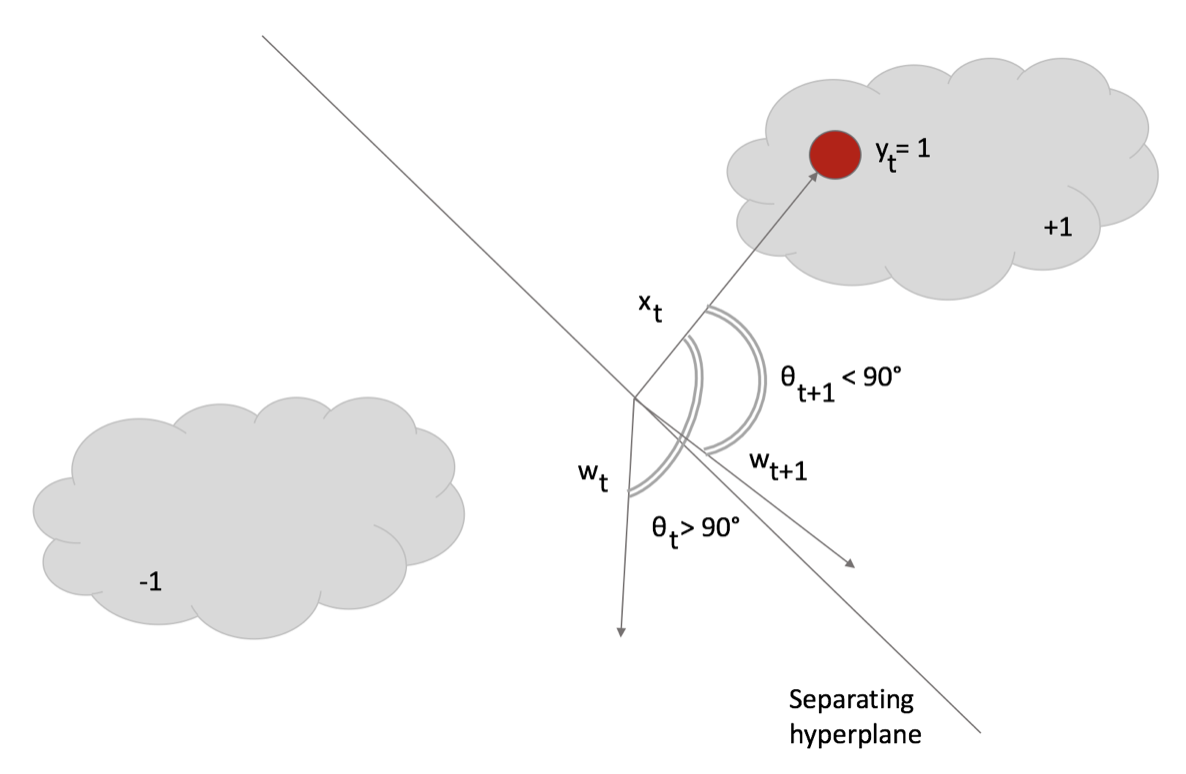
\includegraphics[scale=0.5]{Figure/PAII2.png}
    \caption{Rappresentazione dell'iperpiano e del vettore \textit{w} dopo l'update}
    \label{fig:PAII2}
\end{figure}
\FloatBarrier  


Dopo la rotazione, $\theta <90$ il prodotto punto diventa negativo, quindi il campione è correttamente classificato come $+1$.

L'idea è fornire all'utente un sistema già pre-addestrato che pian piano si adatti alle sue esigenze. Per questo scopo dobbiamo adottare una strategia di transfer-learning / multi-view learning\cite{transfer-learning} (vedi Figura~\ref{fig:approccisens}.

Si vuole addestrare il Customized Sensitiveness Classifier con una multi-view che include sia l'embed (single-view) sia la valutazione del sensitiveness classifier (single-view). Abbiamo utilizzato in particolare la tecnica \textit{early integration}. 

La \quotes{early integration} consiste nel concatenare le view singole cioè le caratteristiche associate all'embed e i risultati in probabilità ottenuti tramite il Topic-specific Sensitiveness Classifier; in questo modo ogni combinazione (concatenazione di due o più viste singole) rappresenta un campione nei set di dati. Quindi abbiamo ottenuto vettori da 514 elementi (512+2) dove i primi 512 elementi sono l'embed della frase e gli ultimi due sono la probabilità associata alla sensibilità negativa e la sensibilità positiva, rispettivamente.

\begin{figure}[h]
    \centering
    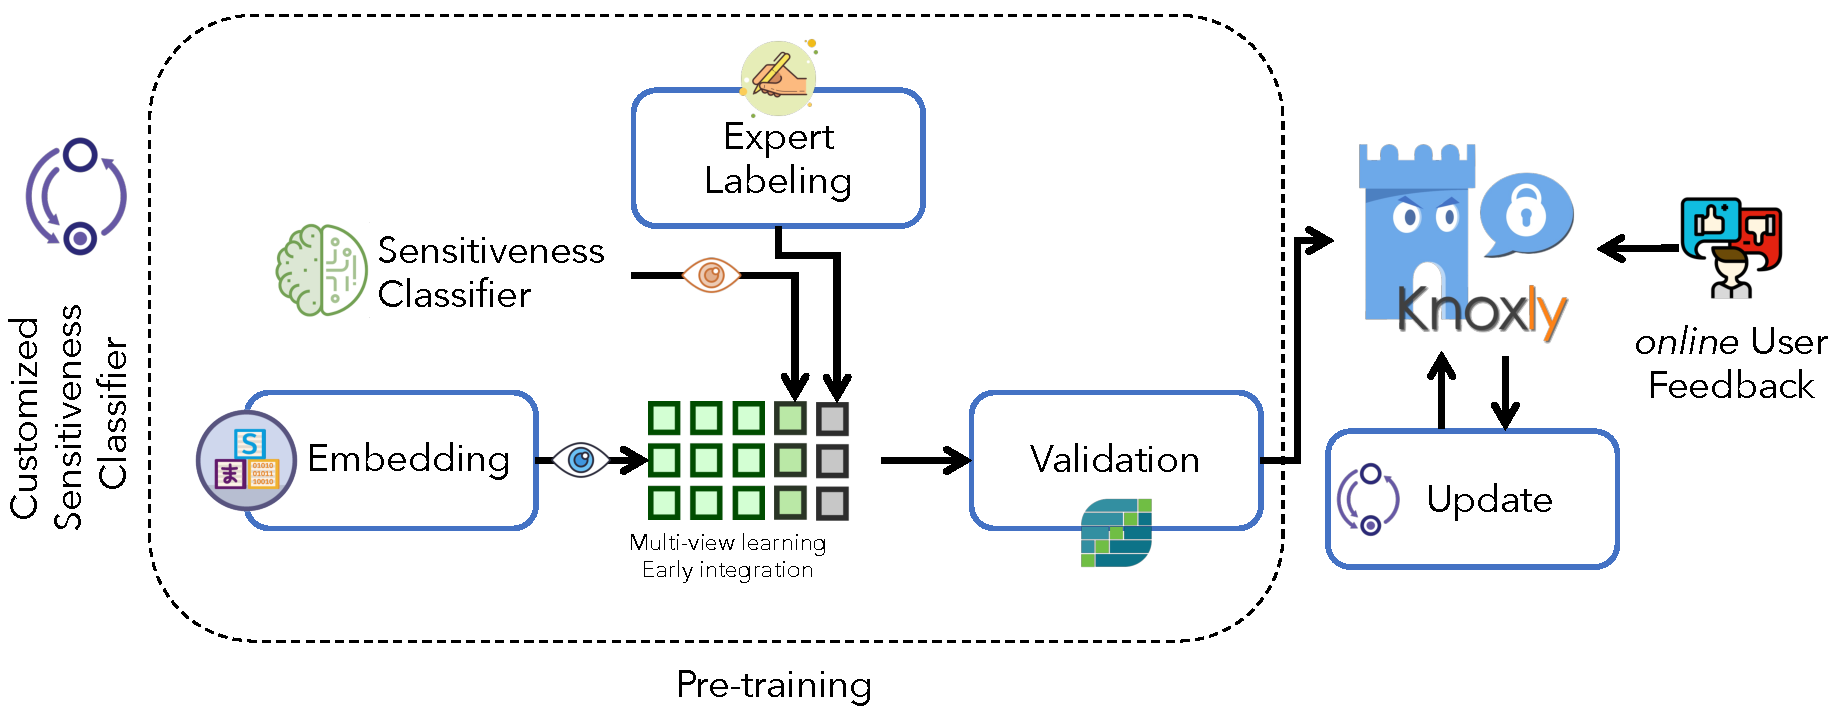
\includegraphics[width=15cm]{Figure/grafici/customized_cropped.pdf}
    \caption{schema riassuntivo del funzionamento del Customized Sensitiveness classifier}
    \label{fig:approccisensCustomized}
\end{figure}
\FloatBarrier

\subsection{Validation}
Abbiamo utilizzato i dataset {\tt ds200.csv} visti in Sezione~\ref{ssec:create_sens_ds} integrati con la valutazione del Topic-specific Sensitiveness Classifier di riferimento. Quindi il dataset {\tt ds200.csv} relativo al topic Health viene integrato con la valutazione di Health Sensitiveness classifier e così via per tutti gli altri.
I dataset sono stati suddivisi, con un approccio stratificato, in un 80\% per il training ed un 20\% per il testing utilizzando la funzione {\tt train\_test\_split} di scikit-learn per Python. Successivamente, il training set è stato oggetto di una 10-fold cross-validation con il metodo {\tt GridSearchCV} in cui abbiamo cercato di ottimizzare il parametro di aggressività $C$. Si osservi però che questo parametro è in realtà molto user-based, ragion per cui il miglior metodo per stimarlo potrebbe essere effettuando uno studio sugli utenti: è possibile che questi preferiscano un classificatore molto aggressivo o, al contrario, siano soddisfatti maggiormente con un apprendimento più lento e graduale. I valori di $C$ provati sono i seguenti: 0.001, 0.01, 0.1, 1, 10, 100. I risultati di questa fase possono essere visti in Tabella~\ref{tbl:testing_Customized}. Il miglior parametro è risultato essere per tutti i casi, $C=0.01$.

\subsection{Testing}
Una volta ottenuto il miglior parametro $C$ di aggressività per ciascun customized sensitiveness classifier procediamo con la fase di testing, in cui valutiamo le prestazioni del classificatore pre-addestrato su un set di dati ancora \quotes{intonso}, il test set, composto dal 20\% dei dati ds200.

\begin{table}[h!t]
\centering

\begin{tabular}{|c|c|c|c|c|}
\hline
\multicolumn{5}{|c|}{\textbf{Accuracy}} \\ \hline
\textbf{Politics} & \textbf{Health} & \textbf{Job} & \textbf{Travel} & \textbf{General} \\ \hline
0.835 & 0.98 & 0.95 & 0.975 & 0.965 \\ \hline
\end{tabular}
\caption{Tabella delle accuracy ottenute dal Customized Sensitiveness Classifier sui vari topic}
\label{tbl:testing_Customized}
\end{table}
\FloatBarrier
I risultati della fase di testing possono essere trovati in Tabella~\ref{tbl:testing_Customized}. Si nota come utilizzando questo approccio le performance del classificatore migliorino sensibilmente rispetto quelle ottenute in Sezione~\ref{sssec:multiclass}.